\documentclass{article}\usepackage[]{graphicx}\usepackage[]{color}
%% maxwidth is the original width if it is less than linewidth
%% otherwise use linewidth (to make sure the graphics do not exceed the margin)
\makeatletter
\def\maxwidth{ %
  \ifdim\Gin@nat@width>\linewidth
    \linewidth
  \else
    \Gin@nat@width
  \fi
}
\makeatother

\definecolor{fgcolor}{rgb}{0.345, 0.345, 0.345}
\newcommand{\hlnum}[1]{\textcolor[rgb]{0.686,0.059,0.569}{#1}}%
\newcommand{\hlstr}[1]{\textcolor[rgb]{0.192,0.494,0.8}{#1}}%
\newcommand{\hlcom}[1]{\textcolor[rgb]{0.678,0.584,0.686}{\textit{#1}}}%
\newcommand{\hlopt}[1]{\textcolor[rgb]{0,0,0}{#1}}%
\newcommand{\hlstd}[1]{\textcolor[rgb]{0.345,0.345,0.345}{#1}}%
\newcommand{\hlkwa}[1]{\textcolor[rgb]{0.161,0.373,0.58}{\textbf{#1}}}%
\newcommand{\hlkwb}[1]{\textcolor[rgb]{0.69,0.353,0.396}{#1}}%
\newcommand{\hlkwc}[1]{\textcolor[rgb]{0.333,0.667,0.333}{#1}}%
\newcommand{\hlkwd}[1]{\textcolor[rgb]{0.737,0.353,0.396}{\textbf{#1}}}%

\usepackage{framed}
\makeatletter
\newenvironment{kframe}{%
 \def\at@end@of@kframe{}%
 \ifinner\ifhmode%
  \def\at@end@of@kframe{\end{minipage}}%
  \begin{minipage}{\columnwidth}%
 \fi\fi%
 \def\FrameCommand##1{\hskip\@totalleftmargin \hskip-\fboxsep
 \colorbox{shadecolor}{##1}\hskip-\fboxsep
     % There is no \\@totalrightmargin, so:
     \hskip-\linewidth \hskip-\@totalleftmargin \hskip\columnwidth}%
 \MakeFramed {\advance\hsize-\width
   \@totalleftmargin\z@ \linewidth\hsize
   \@setminipage}}%
 {\par\unskip\endMakeFramed%
 \at@end@of@kframe}
\makeatother

\definecolor{shadecolor}{rgb}{.97, .97, .97}
\definecolor{messagecolor}{rgb}{0, 0, 0}
\definecolor{warningcolor}{rgb}{1, 0, 1}
\definecolor{errorcolor}{rgb}{1, 0, 0}
\newenvironment{knitrout}{}{} % an empty environment to be redefined in TeX

\usepackage{alltt}
\IfFileExists{upquote.sty}{\usepackage{upquote}}{}
\begin{document}

\begin{knitrout}
\definecolor{shadecolor}{rgb}{0.969, 0.969, 0.969}\color{fgcolor}\begin{kframe}
\begin{alltt}
\hlcom{#GUIA 5}

\hlstd{x} \hlkwb{<-} \hlnum{2}
\hlkwa{if}\hlstd{(x}\hlopt{>}\hlnum{0}\hlstd{) y}\hlkwb{<-}\hlnum{1} \hlkwa{else} \hlstd{y}\hlkwb{<-}\hlnum{0}\hlstd{; y}
\end{alltt}
\begin{verbatim}
## [1] 1
\end{verbatim}
\begin{alltt}
\hlstd{x} \hlkwb{<-} \hlopt{-}\hlnum{1}
\hlkwa{if}\hlstd{(x}\hlopt{>}\hlnum{0}\hlstd{) y}\hlkwb{<-}\hlnum{1} \hlkwa{else} \hlstd{y}\hlkwb{<-}\hlnum{0}\hlstd{; y}
\end{alltt}
\begin{verbatim}
## [1] 0
\end{verbatim}
\begin{alltt}
\hlstd{x} \hlkwb{<-} \hlkwd{c}\hlstd{(}\hlnum{6}\hlopt{:-}\hlnum{4}\hlstd{); x}
\end{alltt}
\begin{verbatim}
##  [1]  6  5  4  3  2  1  0 -1 -2 -3 -4
\end{verbatim}
\begin{alltt}
\hlkwd{sqrt}\hlstd{(x)}
\end{alltt}


{\ttfamily\noindent\color{warningcolor}{\#\# Warning in sqrt(x): Se han producido NaNs}}\begin{verbatim}
##  [1] 2.449490 2.236068 2.000000 1.732051 1.414214 1.000000 0.000000
##  [8]      NaN      NaN      NaN      NaN
\end{verbatim}
\begin{alltt}
\hlkwd{sqrt}\hlstd{(}\hlkwd{ifelse}\hlstd{(x} \hlopt{>=} \hlnum{0}\hlstd{, x,} \hlnum{NA}\hlstd{))}
\end{alltt}
\begin{verbatim}
##  [1] 2.449490 2.236068 2.000000 1.732051 1.414214 1.000000 0.000000
##  [8]       NA       NA       NA       NA
\end{verbatim}
\begin{alltt}
\hlkwd{ifelse}\hlstd{(x} \hlopt{>=} \hlnum{0}\hlstd{,} \hlkwd{sqrt}\hlstd{(x),} \hlnum{NA}\hlstd{)}
\end{alltt}


{\ttfamily\noindent\color{warningcolor}{\#\# Warning in sqrt(x): Se han producido NaNs}}\begin{verbatim}
##  [1] 2.449490 2.236068 2.000000 1.732051 1.414214 1.000000 0.000000
##  [8]       NA       NA       NA       NA
\end{verbatim}
\begin{alltt}
\hlstd{x} \hlkwb{<-} \hlkwd{c}\hlstd{(}\hlnum{2}\hlstd{,} \hlnum{6}\hlstd{,} \hlnum{4}\hlstd{,} \hlnum{7}\hlstd{,} \hlnum{5}\hlstd{,} \hlnum{1}\hlstd{)}
\hlstd{suma}\hlkwb{<-}\hlnum{0}\hlstd{;} \hlkwa{for}\hlstd{(i} \hlkwa{in} \hlnum{1}\hlopt{:}\hlnum{3}\hlstd{) suma} \hlkwb{=} \hlstd{suma}\hlopt{+}\hlstd{x[i]; suma}
\end{alltt}
\begin{verbatim}
## [1] 12
\end{verbatim}
\begin{alltt}
\hlstd{func.cuadratica} \hlkwb{<-} \hlkwa{function}\hlstd{(}\hlkwc{x}\hlstd{)}
\hlstd{\{}
    \hlnum{3}\hlopt{*}\hlstd{x}\hlopt{^}\hlnum{2}\hlopt{-}\hlnum{5}\hlopt{*}\hlstd{x}\hlopt{+}\hlnum{2}
\hlstd{\}}
\hlstd{y} \hlkwb{<-} \hlkwd{func.cuadratica}\hlstd{(}\hlnum{2}\hlstd{);y}
\end{alltt}
\begin{verbatim}
## [1] 4
\end{verbatim}
\begin{alltt}
\hlstd{media} \hlkwb{<-} \hlkwa{function}\hlstd{(}\hlkwc{x}\hlstd{)}
\hlstd{\{}
    \hlstd{n} \hlkwb{=} \hlkwd{length}\hlstd{(x)}
    \hlstd{suma} \hlkwb{<-} \hlnum{0.0}
    \hlkwa{for}\hlstd{(i} \hlkwa{in} \hlnum{1}\hlopt{:}\hlstd{n) suma} \hlkwb{=} \hlstd{suma} \hlopt{+} \hlstd{x[i]}
    \hlstd{media} \hlkwb{=} \hlstd{suma}\hlopt{/}\hlstd{n}
\hlstd{\}}
\hlkwd{save}\hlstd{(media,} \hlkwc{file}\hlstd{=} \hlstr{"media.RData"}\hlstd{)}
\hlkwd{rm}\hlstd{(}\hlkwc{list}\hlstd{=}\hlkwd{ls}\hlstd{(}\hlkwc{all}\hlstd{=}\hlnum{TRUE}\hlstd{))}
\hlkwd{load}\hlstd{(}\hlstr{"media.RData"}\hlstd{)}
\hlstd{x} \hlkwb{<-} \hlnum{1}\hlopt{:}\hlnum{5}\hlstd{;(}\hlkwd{media}\hlstd{(x))}
\end{alltt}
\begin{verbatim}
## [1] 3
\end{verbatim}
\begin{alltt}
\hlstd{y} \hlkwb{<-} \hlkwd{c}\hlstd{(}\hlnum{5}\hlstd{,} \hlnum{NA} \hlstd{,} \hlnum{4}\hlstd{,} \hlnum{9}\hlstd{);(}\hlkwd{media}\hlstd{(y))}
\end{alltt}
\begin{verbatim}
## [1] NA
\end{verbatim}
\begin{alltt}
\hlstd{Seno} \hlkwb{<-} \hlkwa{function}\hlstd{(}\hlkwc{x}\hlstd{)}
    \hlstd{\{}
    \hlstd{y} \hlkwb{=} \hlkwd{sin}\hlstd{(x)}
    \hlkwd{plot}\hlstd{(x, y,} \hlkwc{main}\hlstd{=}\hlstr{"Ejemplo de graficos en R"}\hlstd{,}
         \hlkwc{xlab}\hlstd{=}\hlstr{"x"}\hlstd{,} \hlkwc{ylab}\hlstd{=}\hlstr{"y = Seno(x)"}\hlstd{,} \hlkwc{col}\hlstd{=}\hlstr{"blue"}\hlstd{,} \hlkwc{pch}\hlstd{=}\hlnum{1}\hlstd{)}
\hlstd{\}}
\hlstd{x}\hlkwb{<-}\hlkwd{seq}\hlstd{(}\hlopt{-}\hlstd{pi, pi,} \hlkwc{len}\hlstd{=}\hlnum{100}\hlstd{)}
\hlkwd{Seno}\hlstd{(x)}
\end{alltt}
\end{kframe}
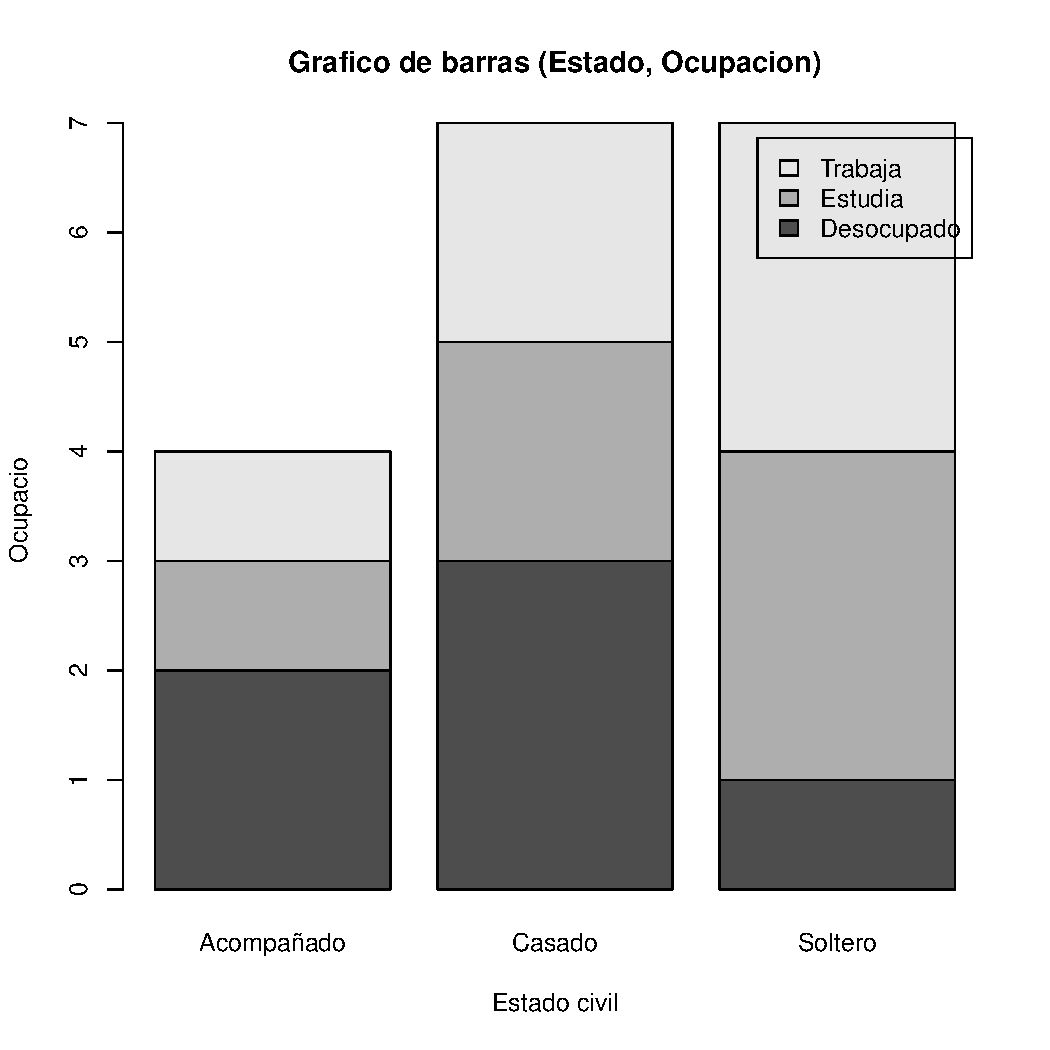
\includegraphics[width=\maxwidth]{figure/unnamed-chunk-1-1} 
\begin{kframe}\begin{alltt}
\hlcom{#Factorial de un muero}
\hlstd{factiorial} \hlkwb{<-} \hlkwa{function}\hlstd{(}\hlkwc{x}\hlstd{)} \hlkwd{prod}\hlstd{(}\hlnum{1}\hlopt{:}\hlstd{x)}
\hlkwd{factorial}\hlstd{(}\hlnum{4}\hlstd{)}
\end{alltt}
\begin{verbatim}
## [1] 24
\end{verbatim}
\end{kframe}
\end{knitrout}



\end{document}
